\chapter{Guía de usuario de la aplicación de control}\label{chap:appendixA}

Este manual pretende instruir al lector que esté interesado en el manejo
del sistema de medida digital desarrollado como parte del proyecto
documentado en esta memoria por medio del software que le sirve de interfaz
para con el usuario. La otra intención que persigue este documento es la de
valer como manual de referencia para futuras consultas. En vistas a
conseguir dichos objetivos, el manual se ha estructurado del siguiente
modo. Por una parte se describen de forma concisa las principales
características funcionales que definen la aplicación como son: la
organización de la interfaz de usuario, la función de los distintos
controles presentes en dicha interfaz, o los tipos de dato que devuelve la
aplicación en sus distintas configuraciones, etcétera. Todo ello acompañado
de una serie de directrices que indican cual es el procedimiento a seguir
para poner en funcionamiento o detener el sistema de medida y activar
correctamente cualquiera de sus funciones. De modo que un usuario que está
aprendiendo a manejar la aplicación puede prepararse leyendo la primera
descripción, que puede ir consultando a medida que aprende los distintos
procedimientos detallados en el manual; al tiempo que se da al usuario
experimentado la posibilidad de consultar cualquier detalle de la
aplicación que no recuerde de forma precisa.


\section{Especificaciones}

A continuación se enumeran brevemente los requisitos necesarios para poder
instalar y utilizar la aplicación de control en un \textsc{pc}. Por un lado
se tienen los requisitos que debe satisfacer un ordenador para que en éste
pueda instalarse la tarjeta de adquisición que, como apunta el segundo
capítulo de la memoria, constituye una parte fundamental del sistema de
medida. Dichos requisitos se enumeran a continuación:

\begin{itemize}
	\item Es necesaria una ranura \textsc{pci} libre en la placa base
		del ordenador.
	\item Para instalar los drivers de la tarjeta, necesarios para que
		exista comunicación entre \sig{matlab} y la \kpci{}, el
		sistema debe ejecutar un sistema operativo Microsoft
		Windows. Estos drivers se encuentran disponibles
		directamente en la web del fabricante.
	\item Puede sustituirse la \kpci{} por una tarjeta compatible de
		características similares manufacturada por el mismo
		fabricante.
\end{itemize}

Por otro lado, para poder utilizar la software de control en el ordenador
en el que se haya instalado la tarjeta de adquisición es necesario,
obviamente, disponer de una copia de \sig{matlab} instalada en el sistema y
de una copia de la propia aplicación, de los ficheros fuente, también
instalados en el disco duro del ordenador. Como explica el
\cref{subsec:conbox}, la interfaz estándar con la que cuenta la tarjeta de
adquisición está diseñada para servir como una vía de comunicación entre
dispositivos de características similares a las de la tarjeta y, en
consecuencia, no está preparada para conectar la tarjeta a sondas con el
fin de explorar circuitos electrónicos; para poder utilizar la tarjeta como
parte del sistema de medida es pues necesario un accesorio que simplifique
esta tarea.


\section{Limitaciones del software}

Este apartado trata de las limitaciones que presenta el software de control
atendiendo al siguiente concepto: allí donde existe la posibilidad de
configurar un parámetro de funcionamiento del sistema de medida se entiende
que el software de control presenta una limitación si priva al usuario de
dicha opción por el mero hecho de emplear la aplicación para interactuar
con el sistema de medida en lugar de haber recurrido a cualquier otro medio
disponible. Este tipo de <<limitaciones>> surgen fundamentalmente debido a
que frente a la multitud de opciones de configuración que presenta el
sistema resulta adecuado representar en la interfaz de usuario únicamente
las más relevantes de cara a realizar una prueba experimental. Se descarta,
por tanto, analizar cualquier limitación de carácter técnico asociada a la
aplicación, principalmente debido a que este tipo de limitaciones las
hereda el software del sistema en el que se ejecuta.

Mencionar que el sistema de medida presenta asimismo sus propias
limitaciones, heredadas por su parte de los distintos subsistemas que lo
integran, limitaciones que inevitablemente se ven reflejadas en la
aplicación de software. Por ejemplo, uno no puede configurar el sistema
desde la aplicación para que muestree señales cuyo nivel de pico a pico sea
superior a 10 Vpp, pues el sistema de por sí no lo permite, ahí la
aplicación no tiene nada que ver. Dentro de este segundo grupo son notables
las limitaciones que derivan del uso de la tarjeta \kpci{} como instrumento
para la adquisición de señales, éstas se encuentran debidamente
documentadas en las \vrefrange{sec:technical}{sec:throughput}, donde el
lector puede consultarlas. Cabe mencionar aquí también que el rendimiento
de la tarjeta es limitado y depende no sólo de como se encuentre
configurada, si no también del nivel de la señal de entrada así como de
otros parámetros.

Por lo demás, este apartado trata únicamente de las limitaciones que son
inherentes a la propia aplicación, que tienen su origen en el planteamiento
de su código fuente y que surgen como parte del proceso de diseño y el
posterior proceso de programación. En el proceso de diseño se ha priorizado
la sencillez a la completitud. De ese modo se explican las decisiones que
han dado lugar a que el software presente las siguientes limitaciones.

\begin{itemize}
	\item El software de control no permite la manipulación directa de
		la cola de muestreo. Únicamente se da acceso a un canal
		que, eso sí, puede vincularse a voluntad (es preciso pausar
		previamente la sesión de adquisición) a cualquier puerto
		físico de la tarjeta, esté configurado en modo diferencial
		o sencillo.
	\item No todas las opciones de configuración de objeto dispositivo
		y de canal se encuentran representadas mediante controles
		en la interfaz de usuario de la aplicación. Eso significa
		que no es posible configurar desde el software esas
		propiedades.
	\item Algunos de los controles de la interfaz se deshabilitan al
		reanudar la sesión de adquisición. Esto impide que se
		produzcan errores si se trata de configurar al vuelo alguna
		propiedad de configuración cuando no está permitido (sólo
		ocurre con un subconjunto de las propiedades) y simplifica
		el diseño de la aplicación.
\end{itemize}

\section{Procedimientos de llamada}

El manejo del software de representación de señales es relativamente
sencillo. Para arrancar el software debe ejecutarse en primer lugar
\matlab{}\footnote{Si se necesita más información con respecto al uso de
\matlab{}, puede consultarse el manual de instrucciones proporcionado por
el desarrollador del software.}. Después debe hacerse una llamada a la
aplicación de control, existen tres modos de hacer esto mismo, todos ellos
explicados con detalle en el manual de usuario de \matlab{}. En lo
fundamental el procedimiento es idéntico a la llamada a una función
implementada en un fichero de código de \matlab{}. De los modos mencionados
son interesantes desde la perspectiva que adopta este manual dos de
ellos.

\begin{itemize}
	\item El primero, quizás más intuitivo, es el modo gráfico, que más
		bien es un compendio de las distintas formas de ejecutar un
		fichero *.m que permite \matlab{}, sólo que aplicado al
		código de una aplicación con interfaz de usuario. Para dar
		un ejemplo, desde el navegador de carpetas de \matlab{}
		puede hacerse click con el botón derecho del ratón en el
		fichero *.m asociado al software (fichero
		\texttt{single\_channel.m}) y seguidamente seleccionar en
		el desplegable que aparece la opción <<ejecutar archivo>>.
	\item Otra forma es la llamada desde la línea de comandos.
		Cerciorándose de que el directorio actual contiene los
		ficheros \texttt{single\_channel.m} correspondiente al
		código y \texttt{single\_channel.fig} correspondiente a la
		distribución de la interfaz puede escribirse en la línea de
		comandos la orden:

		\begin{lstlisting}[gobble=16]
			[handles = ]single_channel[(opciones)]
		\end{lstlisting}

		Siendo la parte entre corchetes del comando opcional.

		Lo interesante de este método es que permite el acceso a
		las propiedades internas y objetos de los que hace uso la
		aplicación de control. De este modo es posible a partir del
		objeto \texttt{handles} tener acceso, por ejemplo, al
		objeto dispositivo que controla la tarjeta de adquisición
		de señales. Además a través de la llamada por línea de
		comandos es posible pasar argumentos para posibles opciones
		relacionadas con las interfaces de usuario.
\end{itemize}


\section{Rutina de inicialización}

De no existir ningún objeto dispositivo asociado a la \kpci{}, la función
de creación presente en la aplicación crea, al iniciarse ésta, un objeto
dispositivo asociado a la \kpci{} o cualquier otra tarjeta fabricada por
\emph{Keithley} soportada por el software e instalada en el \textsc{pc}. En
caso contrario el software hereda uno de los posibles objetos dispositivos
existentes añadiendo un nuevo canal y emite un mensaje de advertencia.

Al cerrar la aplicación se detiene el proceso de muestreo y, si el número
de canales pertenecientes al objeto dispositivo empleado no ha disminuido,
se elimina el canal cuyo orden corresponde al número de canales existentes
al lanzar la aplicación más uno. Es importante remarcar que en ningún caso
se elimina el objeto dispositivo del que se ha hecho uso, ni siquiera
cuando es la aplicación la que lo ha generado. Queda pues en manos del
usuario la tarea de destruir cualquier canal creado por la aplicación de
control y el objeto dispositivo correspondiente en caso de ser necesario.
La forma más sencilla de hacerlo es la que se cita a continuación, que
también eliminará cualquier variable que quedase en el espacio de trabajo
de \matlab{} ---para evitarlo debe llamarse a \texttt{clear} utilizando
como argumentos, separados por espacios entre ellos y del comando, los
nombres de los objetos dispositivos eliminados de la memoria de \matlab{}
que queden en el espacio de trabajo---.

\begin{lstlisting}
	delete(daqfind);	clear;
\end{lstlisting}


\section{Interfaz de usuario}

En la \vref{fig:interface} puede observarse el aspecto general (justo
después de ejecutarse y antes de ser utilizada) que muestra la aplicación
de control. Como puede verse, se ha dividido la interfaz gráfica en
distintos paneles en los que se reúnen los elementos de que consta esta
interfaz. En el primer panel se observan los elementos que permiten
controlar los parámetros de configuración de la tarjeta de adquisición. Un
segundo panel contiene un monitor en el que se representan los resultados
del proceso de adquisición en los modos numéricos o no visuales de
funcionamiento de la aplicación. Además, un subpanel alberga los controles
que permiten, por un lado, gobernar el modo de funcionamiento y, por otro,
el comportamiento de la función de representación.

\begin{figure}
	\begin{center}
		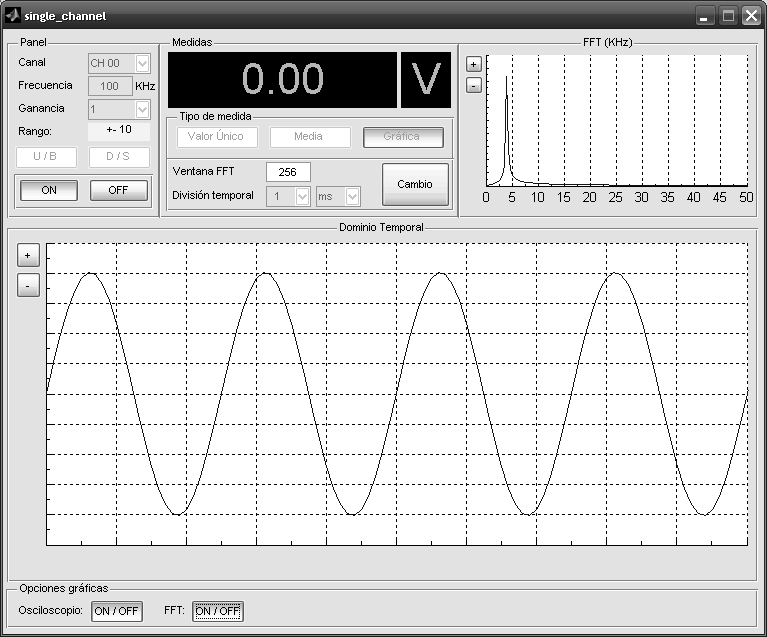
\includegraphics{gis-pfc-appa-01.png}
	\end{center}
	\caption[Aspecto de la interfaz de usuario]{Aspecto de la interfaz
	con controles y gráficos separados por paneles.}
	\label{fig:interface}
\end{figure}

A continuación pueden observarse dos paneles que contienen los espacios de
coordenadas destinados a alojar las representaciones de señal y espectro y
varios grupos de controles, uno por cada espacio de coordenadas, cada uno
de los cuales controla propiedades del espacio de coordenadas al que está
sujeto. Por último, un quinto panel dispone de los mandos necesarios para
habilitar o deshabilitar la representación de señal, espectro o ambos.


\subsection{Funciones asociadas a los controles}

Aquí, en este apartado, se muestran los controles y sus funciones para que
el usuario pueda comprender su funcionamiento. Para facilitar la búsqueda
se ha procedido a agrupar las definiciones empleando como criterio la
pertenencia a mismo panel, es decir, todos los controles que aparecen
reunidos en un mismo panel en la interfaz de usuario se explican en un
mismo cuadro.

\begin{table}
	\centering
	\begin{minipage}{.85\textwidth}
		\begin{description}
			\item[Canal] Determina el puerto físico asociado al
				canal en uso. Se trata de un control
				desplegable que se expande mostrando todos
				los puertos seleccionables.
			\item[Frecuencia] Permite ajustar la frecuencia de
				muestreo. La nueva frecuencia de muestreo
				se limita de forma automática de modo que
				se encuentre entre 1 kHz y la máxima
				frecuencia de muestreo permitida por la
				tarjeta.
			\item[Ganancia] Ajusta el rango de amplificación
				del amplificador de instrumentación
				integrado en la tarjeta. Esto a su vez
				condiciona la amplitud de pico máxima de la
				señal que entra a la \kpci{}. Éste es
				también un control desplegable y muestra el
				conjunto de ganancias posibles.
			\item[Rango] Indicador que presenta el rango en el
				que debe mantenerse la amplitud de la señal
				que entra a la tarjeta para que el
				conversor analógico digital no sature dada
				una configuración de ganancia y método de
				adquisición. Puede consultarse el
				\vref{tab:acqmodes} al respecto.
			\item[Control u/b] Controla el modo de adquisición
				en el proceso de muestreo. El modo de
				adquisición es en la \datx{} una propiedad
				del objeto dispositivo y no del canal.
			\item[Control d/s] Permite configurar el modo de
				terminación correspondiente al canal que se
				controla. De configurarse como diferencial
				el listado de canales que muestra el
				desplegable \textsf{canal} se modifica para
				concordar con esta configuración.
		\end{description}
	\end{minipage}
	\caption[Descripción del primer panel de controles]{Descripción del
	primer panel de controles.}
	\label{tab:first-panel}
\end{table}

El primer panel descrito en el \vref{tab:first-panel} alberga un panel
secundario o subpanel en el que se encuentran ubicados dos controles más.
Estos controles son el control \emph{on} y el control \emph{off} que
respectivamente sirven para iniciar o detener el proceso de muestreo.

El siguiente panel a la derecha con el nombre de \emph{medidas} muestra un
indicador numérico verde en fondo negro que, una vez activado el proceso de
muestreo, si la aplicación se encuentra funcionando en los modos
\emph{valor único} o \emph{media}, presenta el valor que toma la señal en
cada evento. Adicionalmente puede verse un panel más pequeño, \emph{tipo de
medidas}, dentro de este panel. Los elementos que incorpora el subpanel
tipo de medidas vienen explicados en el \vref{tab:second-panel}.

\begin{table}
	\centering
	\begin{minipage}{.85\textwidth}
		\begin{description}
			\item[Tipo de medidas] Representado por tres
				botones: \emph{valor único}, \emph{media},
				y \emph{gráfica}; de los cuales sólo uno
				puede quedar pulsado al mismo tiempo.
				Gobierna el modo de funcionamiento del
				software de control. Los modos de
				funcionamiento de la aplicación de control
				se encuentran explicados al detalle en el
				\vref{subsec:working-modes}.
			\item[Ventana fft] Determina la longitud en número
				de muestras de la ventana empleada para el
				cálculo de la \textsc{fft}. Este control se
				presenta en la forma de cuadro de texto
				editable. El valor introducido en el texto
				es redondeado a la siguiente potencia de
				dos.
			\item[División temporal] Este mando está formado
				por dos controles desplegables. El primero
				de los cuales permite seleccionar un número
				de una secuencia que va de 1 a 400. El
				segundo por su parte sirve para seleccionar
				una escala de unidades: milisegundos o
				microsegundos. El propósito del conjunto es
				controlar la longitud temporal que
				representa el eje de coordenadas del
				espacio de coordenadas en el que se
				representa la señal. Esto que a priori
				parece no repercutir demasiado en el
				funcionamiento del software, adquiere una
				gran importancia dado que el software de
				control se ha diseñado para asemejarse en
				su modo de funcionamiento gráfico a un
				osciloscopio digital. Para más información
				sobre el funcionamiento de los
				osciloscopios digitales consúltese el
				\vref{sec:softdesign}.
			\item[Cambio] Inicialmente la \textsc{fft} de la
				señal se representa en el espacio de
				coordenadas más pequeño, arriba a la
				derecha en la interfaz de usuario, y la
				señal se representa en el espacio de
				coordenadas mayor. Mediante este mando es
				posible reubicar las representaciones de
				señal y transformada de Fourier.
		\end{description}
	\end{minipage}
	\caption[Descripción del segundo panel de controles]{Descripción
	del segundo panel de controles incluido en el panel
	\emph{medidas}.}
	\label{tab:second-panel}
\end{table}

Para terminar existe un panel adicional que incorpora los controles
\emph{osciloscopio} y \emph{fft}. Sendos mandos permiten en el modo de
funcionamiento gráfico habilitar o inhabilitar la representación de la
señal y/o el cálculo y representación de la \textsc{fft} de la señal
respectivamente. Asimismo, cada uno de los paneles en los que se sitúan los
espacios de coordenadas está dotado de dos controles con una etiqueta que
representa los signos matemáticos de la suma y la resta. Estos botones
controlan la escala axial en relación con el eje de ordenadas en el espacio
de coordenadas al que acompañan.


\subsection{Modos de funcionamiento}\label{subsec:working-modes}

Los modos de funcionamiento que soporta el software de control de la
\kpci{} son tres. En el último de ellos, el modo gráfico, la aplicación
consigue simular un osciloscopio digital de acuerdo con los resultados
mostrados en la \vref{sec:working-test}. Se han discutido los pormenores de
este modo de funcionamiento a lo largo del grueso de la memoria, para
evitar reiteraciones innecesarias no volverá a tratarse el tema en este
punto.

El resto de modos de funcionamiento podría catalogarse como modos numéricos
o no gráficos. La razón es que durante el proceso de adquisición el usuario
percibe un valor numérico y no una representación gráfica de la señal si
alguno de estos modos se encuentra activado. Es importante destacar que
estos modos de funcionamiento no son apropiados para el estudio de señales
de alta frecuencia. En situaciones en las que la señal oscila a alta
frecuencia el análisis mediante la aplicación configurada para funcionar en
alguno de estos dos modos aporta información confusa que no debe ser tomada
en cuenta. No obstante, se recomienda encarecidamente su uso de producirse
la situación contraria, aquella en la que la señal analizada oscila con
lentitud. Esto es debido en principio a la naturaleza de los algoritmos en
los que se basan ambos modos de funcionamiento y los resultados que
otorgan.% en cuanto a que aportan en tales circunstancias / en tal caso
% información confusa acerca de la señal / señales / información no
% representativa.

Los modos numéricos de funcionamiento comparten una mecánica similar, en lo
fundamental idéntica, no obstante, diferente en cuanto a implementación. La
idea es programar, antes de que dé inicio el proceso de adquisición, los
eventos relacionados con el objeto dispositivo de la \datx{} de modo que
ocurran periódicamente. Cuando acontece uno de los eventos se obtiene un
número real a partir de una interpretación hecha a partir de la muestra o
muestras adquiridas desde el evento anterior y se escribe éste en el
indicador numérico que forma parte de la interfaz de usuario. Hasta ahí las
coincidencias entre los métodos que ejecuta cada modo de
funcionamiento.% de modo cada cierto número periódico de muestras
% obtenidas se programan

Las diferencias entre el método \emph{valor único} y \emph{media} son las
que siguen:

\begin{itemize}
% 	\item En primer lugar, con el modo valor único se obtiene el valor
% 		de la muestra adquirida justo antes, después de producirse
% 		el evento, mientras que el modo media proporciona la media
% 		aritmética de las muestras obtenidas desde el evento
% 		inmediatamente anterior al actual al ritmo especificado por
% 		el control \textsf{frecuencia}.
	\item En primer lugar, en el modo valor único el software muestra
		en el display\footnote{A partir de la vigésimo tercera
		edición del diccionario de la real academia de la lengua se
		considera correcto decir visualizador e incorrecto decir
		\emph{display}.} el valor correspondiente a la muestra
		obtenida justo después de producirse el último evento,
		mientras que el modo media proporciona la media aritmética
		de las muestras obtenidas desde el evento inmediatamente
		anterior al actual al ritmo especificado por el control
		\textsf{frecuencia}.
	\item Más allá de lo inferido a partir del nombre de los modos,
		estos se diferencian en el criterio empleado en la
		definición del periodo entre eventos y en la herramienta
		que genera dichos eventos. El método valor único emplea el
		reloj interno de la \kpci{} a modo de temporizador, los
		eventos en este modo se programan para que sucedan cada
		cuarto de segundo. Por el contrario el modo media emplea
		una especie de testigo electrónico que implementa la
		\datx{} y que produce un evento cada vez que se adquiere un
		determinado número de muestras definido por el usuario de
		\matlab{}, en este caso el programador, a través de la
		propiedad \textsf{SamplesAcquiredFcnCount}. El número de
		muestras que debe adquirirse antes de que se produzca un
		evento se ha configurado a un valor que queda entre la
		cantidad de muestras que se obtienen en 250 milisegundos a
		la frecuencia de muestreo establecida y un mínimo que
		\matlab{} actualiza al modificarse esta frecuencia.
	\item Por último, cabe hacer mención al procedimiento empleado para
		obtener el valor que se muestra por pantalla. El modo valor
		único emplea la función \texttt{getsample} que extrae una
		única muestra de la tarjeta de adquisición, de este forma
		la tarjeta pasa gran parte del periodo entre eventos en
		reposo. El modo media, por el contrario, utiliza la función
		\texttt{mean} sobre \texttt{getdata} que recupera las
		muestras almacenadas hasta el momento en el buffer en tanto
		que lo borra.
\end{itemize}


\subsubsection[Modos numéricos y señales de alta
frecuencia]{Incompatibilidades entre los modos de funcionamiento numéricos
y el análisis de señales de alta frecuencia}

La razón de que estos modos de funcionamiento no sean apropiados para el
estudio de señales de alta frecuencia es diferente según el modo.

\begin{itemize}
% 	\item El modo valor único extrae una muestra de la señal de manera
% 		periódica. Si consideramos que la señal resultante de este
% 		proceso es el producto entre la señal analizada y un tren
% 		de deltas. Si combinamos el hecho de que la frecuencia de
% 		la señal es superior o muy superior a la frecuencia del
% 		tren de deltas y que posiblemente no sea un múltiplo de
% 		ésta con la certeza de que ambas señales se encuentran
% 		desfasadas en una medida desconocida y que es difícil
% 		seguir un número real que cambia cuatro veces por segundo,
% 		el resultado es una información caótica y poco
% 		representativa de la señal.  % Dependiente del modo pero
% % 		radica en la forma de obtener el número que se muestra por
% % 		pantalla. El primer método aplicado a una señal que oscila
% % 		no en fase con la señal de muestreo hace parecer el
% % 		comportamiento de la señal errático. El segundo, la media
% % 		de muchos periodos de una señal centrada en el origen
% % 		tiende a cero.
	\item El modo valor único extrae una muestra de la señal de manera
		periódica, con un periodo de un cuarto de segundo. Es
		decir, se muestrea la señal a una frecuencia de muestreo de
		4 Hz. Considerando la condición de que la frecuencia de la
		señal muestreada es muy alta, puede considerarse como
		consecuencia la hipótesis de que sea muy superior a la
		frecuencia de muestreo, además es poco probable que la
		primera sea un múltiplo de la segunda. Si se combina esta
		suposición con la certeza de que el instante en el que
		empieza el muestreo no coincide con el instante en el que
		se origina la señal, puede llegarse a la conclusión de que
		la información presentada en el visor es, empleando el modo
		valor único en el análisis de señales rápidas, caótica,
		cuanto menos confusa y poco representativa de la señal.
% 		ambas frecuencias pueden no estar relacionadas por una
% 		razón de multiplicidad. Si combinamos el hecho de que la
% 		frecuencia de la señal muestreada es muy superior a la
% 		frecuencia de muestreo, con la posibilidad probable de que
% 		la frecuencia de la señal no sea un múltiplo de la
% 		frecuencia de muestreo, con la certeza de que el instante
% 		en el que empieza el muestreo no coincide con el instante
% 		en el que se origina la señal.
	\item En el caso del modo media ocurre que la media de una cantidad
		determinada de periodos de una señal periódica tiende más a
		cero cuanto más periodos de la señal se estiman al calcular
		la media. Por tanto, si la frecuencia de la señal es mucho
		mayor que la frecuencia con la que se actualiza el valor
		numérico mostrado por pantalla, y ésta también está en
		torno a 4 Hz, el valor que se obtiene es el cero.
\end{itemize}

No es que el modo de funcionamiento gráfico de la aplicación de control
carezca de utilidad en el análisis de señales de baja frecuencia, si no que
carece de utilidad práctica. Debe recordarse al lector que el modo de
funcionamiento gráfico de la aplicación sobre la que trata este manual
pretende emular un osciloscopio digital en su modo de funcionamiento
gráfico y, como consecuencia, este modo de funcionar adolece de los
problemas propios de este tipo dispositivos como, por ejemplo, el que se
expone en este párrafo. El modo de representación que adopta un
osciloscopio digital para representar señales lentas es el modo de
representación continuo, dada la incapacidad de la función de disparo del
modo convencional de trabajar con este tipo de señales \footnote{Esto queda
suficientemente explicado en el \vref{subsec:digosc}.}. Este modo no aporta
información visual precisa sobre la frecuencia de la señal analizada ni
sobre su valor de pico a pico. Por si fuera poco dada la implementación que
se le ha dado en esta aplicación consume muchos más recursos que el modo de
representación convencional\footnote{De hecho en las pruebas de software
que se han realizado para este proyecto el modo de representación continuo
no funciona excepto en el modo de depuración de errores pausando la
ejecución del software, si bien es cierto las pruebas se realizaron con un
\textsc{pc} poco actualizado.}. Y, como es obvio, el modo gráfico
independientemente del modo de representación adoptado necesita más
recursos de los que requieren el resto de modos de funcionamiento.

Es por esta razón por la que los modos numéricos obtienen un mayor
protagonismo en el análisis de señales de baja frecuencia, porque aportan
una información lo bastante buena, comparable a la que proporciona el modo
gráfico, y consumen menos recursos que esta alternativa.
